\documentclass[final]{beamer}

\mode<presentation>
{
  \usetheme{hiitposter}
}
%\graphicspath{{imgs/}}
\usepackage{amsmath,amsthm, amssymb,mathrsfs}
\usepackage{color}
\usepackage{times}
\usepackage{subfigure}
\usepackage{bm}
\usepackage{url}
\usepackage[numbers]{natbib}
\usepackage[orientation=portrait,size=a0,scale=1.4,debug]{beamerposter}
\usepackage{blkarray}        
%\usepackage[orientation=portrait,width = 91 ,height = 122 ,scale=1.39,debug]{beamerposter} 
%\setbeamerfont{itemize/enumerate body}{size={\fontsize{25}{31}}}
%\setbeamerfont{itemize/enumerate subbody}{size=\footnotesize}

\graphicspath{{../qNML_images/}}

\def\newblock{\hskip .11em plus .33em minus 3.07em}

\definecolor{DRed}{rgb}{0.8,0.6,0.6}
\definecolor{DGreen}{rgb}{0.6,0.7,0.6}
\definecolor{BRed}{rgb}{0.7,0,0}
\definecolor{BGreen}{rgb}{0,0.7,0}

\newcommand{\myred}[1]{{\color{BRed}#1}}
\newcommand{\mygreen}[1]{{\color{BGreen}#1}}


\newcommand{\heading}[1]{\alert{\large #1}\\}
\definecolor{myPurple}{RGB}{174, 206, 195}
%\definecolor{myPurple}{RGB}{165,206,190}


\usepackage{textpos}
\usepackage{fancybox}
\setlength{\fboxsep}{12pt}
%\usepackage{mathtools}
\usepackage{empheq}

\theoremstyle{plain}
\newtheorem{assumption}{Assumption}

\definecolor{myblue}{rgb}{.85, .85, 1.0}

%%%%%%%%%%%%%%%%%%%%%%%%%%%%%%%%%%%%%%%%
\newlength\mytemplen
\newsavebox\mytempbox

\makeatletter
\newcommand\mybluebox{%
    \@ifnextchar[%]
       {\@mybluebox}%
       {\@mybluebox[0pt]}}

\def\@mybluebox[#1]{%
    \@ifnextchar[%]
       {\@@mybluebox[#1]}%
       {\@@mybluebox[#1][0pt]}}

\def\@@mybluebox[#1][#2]#3{
    \sbox\mytempbox{#3}%
    \mytemplen\ht\mytempbox
    \advance\mytemplen #1\relax
    \ht\mytempbox\mytemplen
    \mytemplen\dp\mytempbox
    \advance\mytemplen #2\relax
    \dp\mytempbox\mytemplen
    \colorbox{myblue}{\hspace{1em}\usebox{\mytempbox}\hspace{1em}}}

\makeatother
%%%%%%%%%%%%%%%%%%%%%%%%%%%%%%%%%%%%%%%%
\makeatletter
\newcommand\mathcircled[1]{%
  \mathpalette\@mathcircled{#1}%
}
\newcommand\@mathcircled[2]{%
  \tikz[baseline=(math.base)] \node[red,draw,circle,inner sep=1pt] (math) {$\m@th#1#2$};%
}
\makeatother


\title{Quotient Normalized Maximum Likelihood Criterion for Learning Bayesian Network Structures}
\author{Tomi Silander$^1$, Janne Lepp{\"a}-aho$^2$, Elias J{\"a}{\"a}saari$^2$, and Teemu Roos$^2$}
\institute{$^{1}$ NAVER LABS Europe, France \\ 
$^{2}$ HIIT / Department of Computer Science, University of Helsinki, Finland}

\begin{document}
\begin{frame}{}
\vskip-1.0ex

{
\setbeamercolor{block body}{bg=myPurple}
\begin{block}{Abstract}
	\large
  	We introduce an information theoretic criterion for Bayesian network
  	structure learning which we call quotient normalized maximum
	likelihood (qNML). In contrast to the closely related factorized
	normalized maximum likelihood criterion, qNML satisfies the property
	of score equivalence. It is also decomposable and completely free
	of adjustable hyperparameters. For practical computations, we identify
	a remarkably accurate approximation proposed earlier by Szpankowski
	and Weinberger. Experiments on both simulated and real data
	demonstrate that the new criterion leads to parsimonious models with
	good predictive accuracy.
\end{block}
}

\begin{block}{Background: Structure Learning of Bayesian Networks}
\begin{columns}[T]
   \begin{column}{0.3\textwidth} % first column {{{
     \heading{Bayesian Networks}
     \vspace*{12pt}
     \begin{itemize}
     \setlength\itemsep{1em}
     \item Provide a compact way to represent a joint distribution over a random vector $X = (X_1, \ldots , X_d)$. 
     %\item Here, each $X_i$ is a categorical random variable.
     \item Consist of:
     \begin{itemize}
     \item[1.] A Directed acyclic graph $G$ which encodes the dependencies between the components of $X$.
     \item[2.] Parameters $\theta = (\theta_1,\ldots,\theta_d)$, where $\theta_i$ denotes the parameters of the conditional distribution of $X_i$ given its parents $G_i$. 
     \end{itemize}
     \item Decomposition: $P(X \mid G, \theta) = \prod_{i=1}^dP(X_i\mid X_{G_i},\theta_i)$
     \end{itemize}     
   \end{column}
  
   \begin{column}{0.005\textwidth}\linethickness{0.3ex} % separator {{{
      \color{myPurple} \line(0,1){450}
   \end{column} % }}}
   
   \begin{column}{0.25\textwidth} % second column {{{
     \heading{Structure Learning}
     \vspace*{12pt}
     \begin{itemize}
     \setlength\itemsep{1em}
     \item[Data:] Each $X_i$ is a categorical variable. We observe $n$ independent samples of $X$ which are collected in a data matrix $D$ of size $n\times d$. 
     \item[Goal:] We consider a \textit{score-based} approach and seek a graph $G$ that maximizes a scoring function which evaluates how well a given graph fits the observed data.
     \item Some scoring functions: BIC, BDeu and fNML. 
   	 \end{itemize}
   \end{column}
  
   \begin{column}{0.005\textwidth}\linethickness{0.3ex} % separator {{{
      \color{myPurple} \line(0,1){450}
   \end{column} % }}}
   \begin{column}{0.3\textwidth}% third column {{{
     \heading{Scoring Functions}
     \begin{itemize}
	 \vspace*{12pt}
	 \setlength\itemsep{1em}     
     \item[BDeu] Bayesian marginal likelihood based on Dirichlet priors. Depends on a single 
     hyperparameter $\alpha >0$ called equivalent sample size. 
     \item[BIC] Maximized log-likelihood with penalty $\frac{k}{2}\log n$, where $k$ is the number of free parameters in the network. 
     \item[fNML] Factorized Normalized Maximum likelihood. Maximized log-likelihood with penalty defined via \textit{regret} functions.
     \end{itemize}
     
   \end{column} % end of first column }}}
\end{columns}
\end{block}


\begin{block}{Quotient Normalized Maximum Likelihood Criterion}
\begin{columns}[T]

	\begin{column}{0.34\textwidth} % first column {{{
   		\heading{Motivation}
   		\begin{minipage}{0.49\textwidth}
   			\vspace*{12pt}
		   	\textcolor{teal}{BDeu}
			\begin{itemize}	    
		    \item Is very sensitive to the choice of the hyperparameter $\alpha$ \cite{cosco.uai07}.
		    \item Is not \textit{regular} \cite{Suzuki2017} (can be shown in certain situations to favour too complex models over simpler) 
		    \end{itemize}
		    \vspace*{12pt}
		    \textcolor{teal}{fNML}
			\begin{itemize}	    
		    \item Is not score equivalent: the graphs expressing the same independence statements are not scored equally.
		    \item Learned structures are often rather complex, which hampers their interpretation.
		    \end{itemize}		    
	
   		\end{minipage}
   		\begin{minipage}{0.49\textwidth}		   
		   \phantom{why vspace* does nothing??}
		   %\vspace*{12pt} 
		   \textcolor{teal}{BIC}
		    \begin{itemize}
		    \item Appears to
		require large sample sizes in order to identify appropriate
		structures \cite{cosco.pgm08a,Liu2012}. 
			\end{itemize}  
			
			
			\begin{figure}
		  	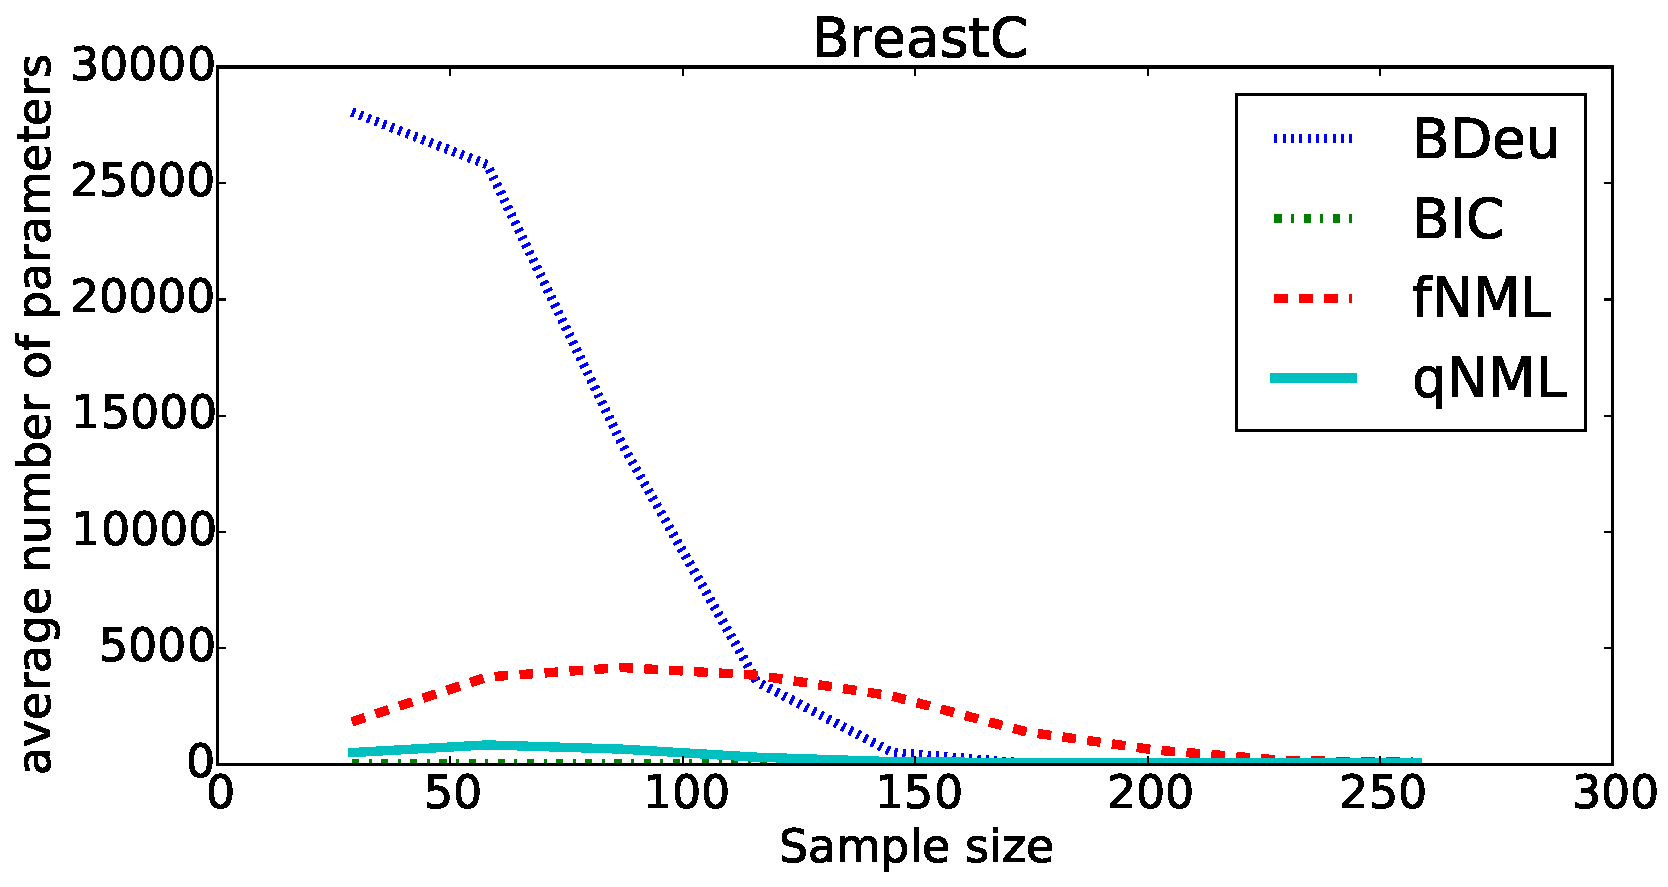
\includegraphics[width=\textwidth]{breast_cancer_npmean.pdf}
		  	\caption{Number of parameters as a function of sample size for Breast Cancer (UCI) data.}
		  	\end{figure}
   		
   		\end{minipage}
   		
   		\vspace*{12pt}
   		
   		\shadowbox{
		\parbox{0.97\textwidth}{
		\vspace*{12pt}
		The quest for a model selection criterion that would yield \textbf{more parsimonious}, \textbf{easier to interpret}, but still \textbf{predictive} Bayesian networks structures is one of the main motivations for this work.
		\vspace*{12pt}
		}}  
		
  
   	\end{column}
   
   \begin{column}{0.005\textwidth}\linethickness{0.3ex} % separator {{{
      \color{myPurple} \line(0,1){810}
   \end{column} % }}}
   
   \begin{column}{0.3\textwidth} % second column {{{
	\heading{qNML: Idea}
	\vspace*{12pt}
	\begin{itemize}
	\item Following the \textit{MDL-principle}, we would like to pick a model $G$ maximizing

	\begin{equation}
	\log P_{NML}(D;G) = \underbrace{\log P(D \mid \hat\theta , G)}_{\text{Maximized log-likelihood}} - \underbrace{\log \sum_{D'}P(D' \mid \hat  \theta,G)}_{:= \text{ regret. } \textbf{Intractable!}}, \notag
	\end{equation}%where $\hat\theta$ denotes the maximum likelihood parameters.

	\item However, for \textbf{a single categorical data vector}, regret and one dimensional $P^1_{NML}$-code can be computed.
	%\item In $P^1_{NML}$, regret depends on $N$, the length of the categorical data vector $D_i$ and $r_i$, the number of possible values for corresponding variable $X_i$. 
	%\item Justification from \textit{Minimum description length} principle.
	\item \textbf{Trick}. Recall factorization w.r.t. graph $G$:
	$$
	P(D\mid G) = \prod_{i = 1}^{d}P(D_i \mid D_{G_i}) = \prod_{i = 1}^{d}\frac{P(D_{i,G_i})}{P(D_{G_i})}
	$$
	\item Assume there are \textbf{no independencies} among $G_i$. Now, $D_{i,G_i} = $
	\vspace*{12pt}
	\end{itemize}
	\begin{minipage}{0.45\textwidth}
	\begin{align*}
	\begin{blockarray}{c|ccc}
	D_i\phantom{s} & \phantom{..}  & D_{G_i} & \phantom{..}\\
	\begin{block}{(c|ccc)}
  	1 & 1 & 1 & 1  \\
  	0 & 1 & 0 & 0 \\
  	1 & 1 &0 & 0  \\
  	1 & 1 & 1 & 1  \\
	\end{block}
	\end{blockarray} 
	\ \to \ 
	\begin{blockarray}{c}
	\phantom{...}\\
	\begin{block}{(c)}
  	0   \\
  	1  \\
  	2  \\
  	0   \\
	\end{block}
	\end{blockarray}
 	\end{align*}
	\end{minipage}\quad
	\begin{minipage}{0.45\textwidth}
	\shadowbox{
	\parbox{\textwidth}{
	\vspace*{12pt}
	\begin{itemize}
	\item We can treat $D_{i,G_i}$ and $D_{G_i}$ as values of single variables!
	\item $P(D_{i,G_i})$ and $P(D_{i,G_i})$ can be modeled using $P_{NML}^1$-code.
	\end{itemize}}}  
	\end{minipage}
	
   \end{column}
   
   \begin{column}{0.005\textwidth}\linethickness{0.3ex} % separator {{{
      \color{myPurple} \line(0,1){810}
   \end{column} % }}}
   
   
   \begin{column}{0.25\textwidth}% third column {{{
   
   	\heading{qNML: Definition \& Properties}
   	\vspace*{12pt}
   	Definition of qNML score:
    	\begin{empheq}[box={\mybluebox[4pt][4pt]}]{equation}	    		
	s^{qNML} := \sum_{i = 1}^d \log \frac{P^1_{NML}(D_{i,G_i})}{P^1_{NML}(D_{G_i})},\notag
	\end{empheq}$\log P^1_{NML}(D) = \log P(D \mid \hat{\theta}) - reg(n,r).$
	
	\begin{itemize}
	 \item $D$ is understood as  $n$ observations on single categorical variable with $r$ possible values.
	\item Accurate approximation for $reg(n,r)$ from \cite{Szpankowski2012}:
	\begin{align*}
    reg(n, r) &\approx  n\left(\log{\alpha} + (\alpha + 2) \log{C_\alpha} - \frac{1}{C_\alpha}\right) \\ 
    &- \frac{1}{2} \log{\left(C_\alpha + \frac{2}{\alpha}\right)},
	\end{align*}
where $\alpha = \frac{r}{n}$ and $C_\alpha = \frac{1}{2} + \frac{1}{2} \sqrt{1 + \frac{4}{\alpha}}$.
	\end{itemize}
	
	\vspace*{12pt}
	\shadowbox{\parbox{0.85\textwidth}{
	\vspace*{12pt}
	\textbf{qNML score is:}
	\begin{itemize}	
	\item \textcolor{teal}{\textbf{hyper-parameter free}}
	\item \textcolor{teal}{\textbf{consistent}}
	\item \textcolor{teal}{\textbf{score equivalent}}
	\item \textcolor{teal}{\textbf{regular}}
	\item \textcolor{teal}{\textbf{it equals NML for many models.}}
	%\item qNML agrees with NML for every network composed of fully connected sub-graphs.
	\end{itemize}}}
	
   \end{column} 
   
   
   
\end{columns}
\end{block}

\begin{block}{Experimental Results}
  \begin{columns}[T]
    \begin{column}{0.35\textwidth}
      \heading{Structure Learning}
      
	  \begin{minipage}{0.45\textwidth}
	  \begin{figure}[h]

		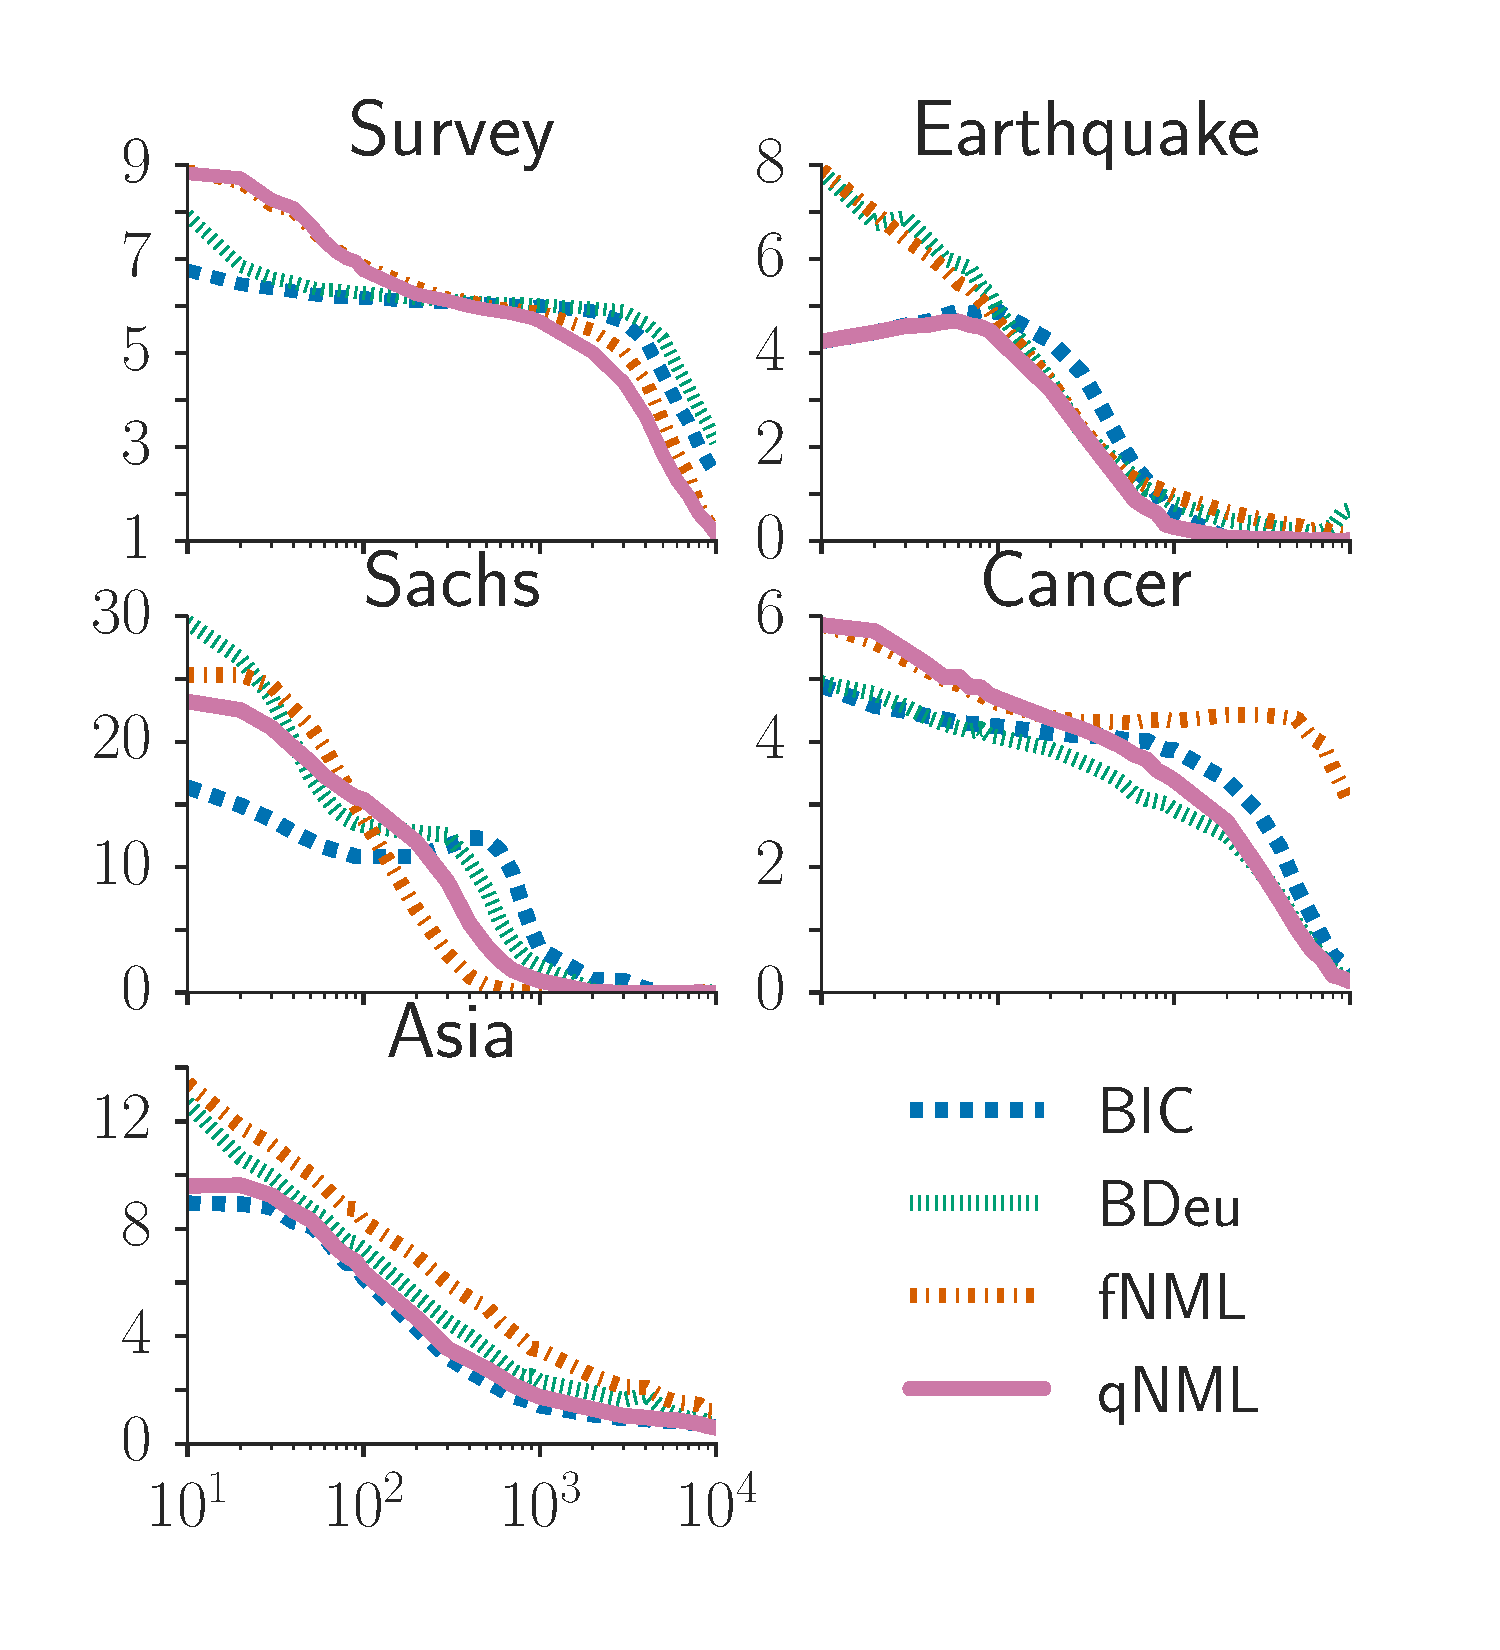
\includegraphics[width=\columnwidth]{shd_all.pdf}
		\caption{SHD as a function of sample size.}
		\label{fig:all_shd}
		\end{figure}
	  \end{minipage}
	  \begin{minipage}{0.45\textwidth}
	  \begin{itemize}
	  \item Data generated from real world DAG structures.
	  \item Exact DP structure learning algorithm.
	  \end{itemize}
	  \begin{figure}[h]
		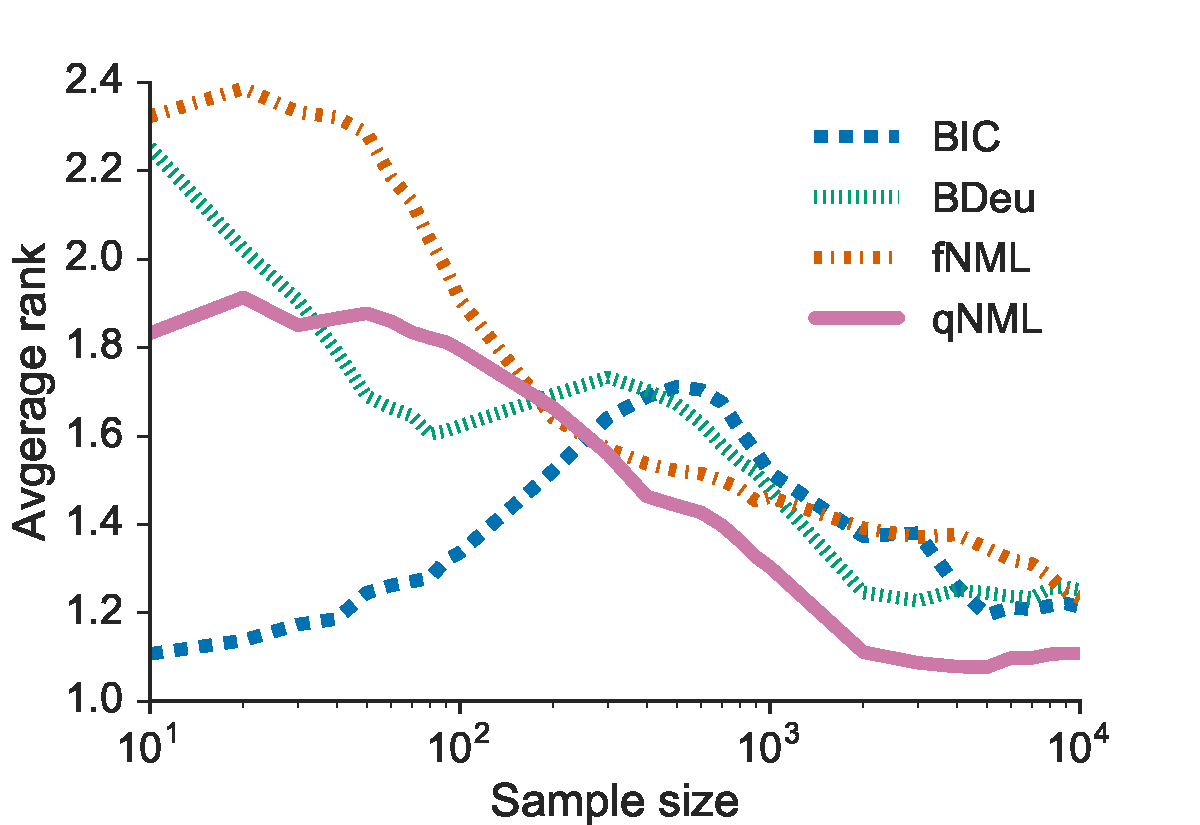
\includegraphics[width=\columnwidth]{shd_rank_all.pdf}
		\caption{Average ranks for each score.}
		\label{fig:all_shd}
		\end{figure}
	  \end{minipage}
	  
	\vspace*{12pt}
	%\textbf{qNML seems overall a safe choice in structure learning, especially with moderate and large sample sizes!} 
    \end{column}
   \begin{column}{0.005\textwidth}\linethickness{0.3ex}
      \color{myPurple} \line(0,1){590}
   \end{column} % }}}
   
    \begin{column}{0.23\textwidth}
    \heading{Prediction}
      
    \end{column}
    
    \begin{column}{0.005\textwidth}\linethickness{0.3ex} % separator {{{
      \color{myPurple} \line(0,1){590}
   \end{column} % }}}
    \begin{column}{0.3\textwidth}
    \heading{Conclusions}

    \end{column}
  \end{columns}
\end{block}

\vskip-1.0ex
\begin{columns}[T]
  \begin{column}{0.63\paperwidth}
\begin{block}{References} %{{{
%\scriptsize
\tiny
{
\bibliographystyle{apalike}
\bibliography{../cosco}
}
\end{block} %}}}
  \end{column}
  \begin{column}{0.33\paperwidth}
\begin{block}{Acknowledgements} %{{{
%\scriptsize
\tiny
{
J.L., E.J. and T.R. were supported by the Academy of Finland (COIN CoE and Project \textsc{TensorML}). J.L. was supported by the DoCS doctoral programme of the University of Helsinki.
}
\end{block} %}}}
  \end{column}
\end{columns}
\end{frame}
\end{document}
 
